\chapter{Project Progress}\label{ch:progress}

Previously in thesis A we elected Minigent as the place to design our new recursive types for Cogent.
Our design was to introduce a new recursive parameter to Minigent's boxed records, in order to allow
for recursively nested data structures. These data structures would be strictly positive as per
definition \autoref{def:sp}, to prevent the programmer constructing infinitely recursive
objects that would lead to termination issues, thus allowing for ease of verification in
the Isabelle embedding.

Work has been completed to incorporate the design into the parser, lexer and reorganiser compiler phases of
Minigent, and work has begun work on integrating updatin the type checking phase.
In addition to the existing suite of tests in the Minigent compiler, additional tests have 
been added to test the newly added extension.

\todo{I'm starting to think this isn't very relevant to the thesis report, let alone the project. Remove?} \\
In order to increase my work efficiency, I created an extension in VSCode that provides syntax highlighting
for both Cogent and Minigent files, which allowed for an easier experience when constructing Minigent programs,
and hence made it easier to write tests for new features.

My work has progressed according to my thesis A schedule, as in \autoref{fig:thesisATimeline}. However, due to 
new discoveries \todo{$<$- rephrase that } for the work on the type checker, my plan has changed for 
thesis C to allow more time for extensions, which are outlined in \autoref{ch:plan}.

\section{Parser and Lexer}

The Minigent lexer and parser now accepts a new recursive parameter extension to boxed records. 
This syntax extends the grammar for types in Minigent, as described in \autoref{fig:recursivetypegrammar}.

This new syntax is backwards compatible with the previous record syntax, so records without this new
syntax in old code will not have to be changed in order for the change to be implemented.


\begin{figure}
    \centering
    \begin{align*}
        \text{types}\quad \tau\;
            ::&= \dots\; |\; [\textbf{mu}\; t]\; \{ \overline{f_i^n\; \tau_i} \} \\
    \end{align*}
    \todo{is there a better way to describe the optional mu $t$ other than writing the two options explictly? [ ] feels dodgy}
    \caption{The new syntax for the type of a boxed record, featuring our recurive parameter $t$}
    \label{fig:recursivetypegrammar}
\end{figure}

\todo{Should I talk about the code I wrote here? Feel this section is very short on a high level.}

\section{Reorganiser}

In the reorganiser, a strict positivity check has been added to prevent the construction of infinitely
recursive objects. This check recursively evaluates all of the functions in a Minigent program, and
checks that their types do not contain a non-strictly positve type. This check also accounts for the
shadowing of recursive parameter variables, in the event a nested boxed record declaration's recursive
parameter shadows the parent record's parameter. These new recursive parameters are now distinguished from
regular type variables, and the reorganiser no longer counts them as type variables.

Functions that also call themselves successfully typecheck as their type signature provides enough information
to check the argument passed to the function, so basic recursion typechecks as expected.

\todo{Unused recursive parameter variables? I could implement this pretty quickly but not sure if we want it}

\section{Type Checker}
\label{sec:typecheckingprogress}

During the typechecking phase, originally we planned to implement two primitives into Minigent to allow referencing
recursive structures; the rules \textsf{roll} and \textsf{unroll} (see \autoref{def:rollunroll}), to insert into and take from recursive structres respectively.

\textsf{roll} works by expanding a recursive parameter 
in the type of a structure by replacing it with the entire type it is nested in - this `adds' one 
layer of recursion to the object. In a list, this would correspond to expanding the type parameter
that is nested in the list to make the list one layer longer on the type level, as in \autoref{fig:rollexample}.

\textsf{unroll} works the opposite way, by removing a layer of recursion from the object. In our
list example, this corresponds to collapsing one layer of our nested list occurence into the
recursive parameter, as in \autoref{fig:unrollexample}. 

\begin{figure}
    \centering
    \begin{align*}
        \infer{
            \Gamma \vdash \textbf{roll } x : \textbf{mu } \textit{t}.\; \tau
        }{
            \Gamma \vdash x : \textbf{mu } \textit{t}.\; \tau[ t := \tau]
        }
        && \infer{
            \Gamma \vdash \textbf{unroll } x : \textbf{mu } \textit{t}.\; \tau[ t := \tau]\; 
        }{
            \Gamma \vdash x : \textbf{mu } \textit{t}.\; \tau
        }
    \end{align*}
    \caption{The rules for roll and unroll}
    \label{def:rollunroll}
\end{figure}

\begin{figure}
    \centering
    \begin{align*}
        \infer{
            \Gamma \vdash \textbf{roll } x : \textbf{mu } \textit{t } \{ \text{ deref}: \langle \text{ Nil } \vert \text{ Cons } \{ \text{data}: a, \text{rest}: {\color{red} t} \}\textit{\#} \rangle \} 
        }{
            \Gamma \vdash x : \textbf{mu } \textit{t } \{ \text{ deref}: \langle \text{ Nil } \vert \text{ Cons } \{ \text{data}: a, \text{rest}: {\color{red} \pi} \}\textit{\#} \rangle \} 
        }
    \end{align*}
    \caption{Rolling a list, where: \newline \protect\phantom{Figure x.x:} $\pi = \textbf{mu } \textit{t } \{ \text{ deref}: \langle \text{ Nil } \vert \text{ Cons } \{ \text{data}: a, \text{rest}: t \}\textit{\#} \rangle \}$}
    \label{fig:rollexample}
\end{figure}

\begin{figure}
    \centering
    \begin{align*}
        \infer{
            \Gamma \vdash \textbf{unroll } x : \textbf{mu } \textit{t } \{ \text{ deref}: \langle \text{ Nil } \vert \text{ Cons } \{ \text{data}: a, \text{rest}: {\color{red} \pi}  \}\textit{\#} \rangle \} 
        }{
            \Gamma \vdash x : \textbf{mu } \textit{t } \{ \text{ deref}: \langle \text{ Nil } \vert \text{ Cons } \{ \text{data}: a, \text{rest}: {\color{red} t} \}\textit{\#} \rangle \} 
        }
    \end{align*}
    \caption{Unrolling a list, where: \newline \protect\phantom{Figure x.x:} $\pi = \textbf{mu } \textit{t } \{ \text{ deref}: \langle \text{ Nil } \vert \text{ Cons } \{ \text{data}: a, \text{rest}: t \}\textit{\#} \rangle \}$}
    \label{fig:unrollexample}
\end{figure}

Normally we would need to implement these primitives and then later use type inference so that
the programmer would not need to explicitly roll or unroll a structure However,
in Minigent we may bypass adding these new primitives alltogether by using the primitives
that already exist in the language. Minigent's \textsf{take} and \textsf{put} are primitives to
operate on boxed records which our recursive types inhabit, so we may facilitate the behaviour
of roll and unroll by adding it into take and put when we perform operations on a recursive record.

\todo{\LaTeX\; up the equations for putting/taking, further describe}

\section{Testing}

\todo{Remove the screenshots and write \LaTeX}

A suite of tests has been added to the existing Minigent test suite in order to test the new extension's 
expected behaviour.

The tests aim to test the intended functionality of our recursive types, including constructing and manipulating
recursive data structures (such as lists), as well as recursive functions that do not use our recursive types 
(such as functions recursing on U32 integers, etc.).

An example of such a test is seen in \autoref{fig:test1}, which constructs an empty list given the presence
of an external allocation function.

\begin{figure}
    \centering
    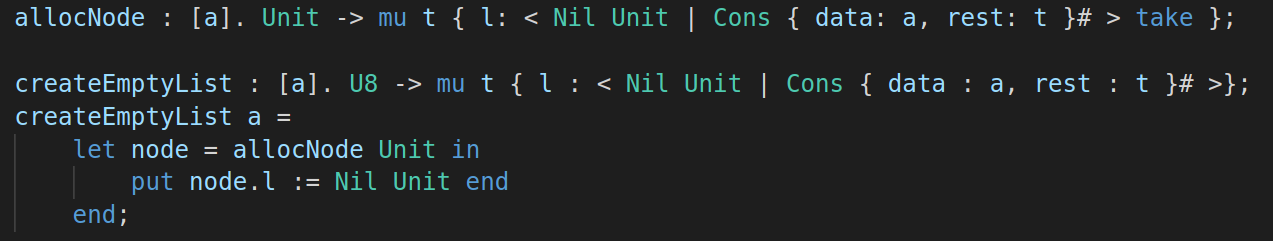
\includegraphics[width=\linewidth]{content/test1.png}
    \caption{Testing the construction of an empty list \todo{Replace images with LaTeX'd code?}}
    \label{fig:test1}
\end{figure}

These tests also test the intended effects of our new types, such as the strict positivity guarantee they provide
and their interaction with the existing type system. Whilst the existing tests test the backwards compatability of
record types, our new tests check that no recursive parameters are used non-strictly positive, that shadowing of recursive
parameters behaves as intended, and that recursive parameters are seperate from quantified type variables.

\autoref{fig:test2} shows a function with a non-strictly positive occurence of a recursive parameter nested in 
a negative position as the return type of a a function that is an argument. This program is rejected by the reorganiser
as shown in \autoref{fig:test2result}, which shows the recursive parameter $t$ that occurrs non-strictly positive.

\begin{figure}
    \centering
    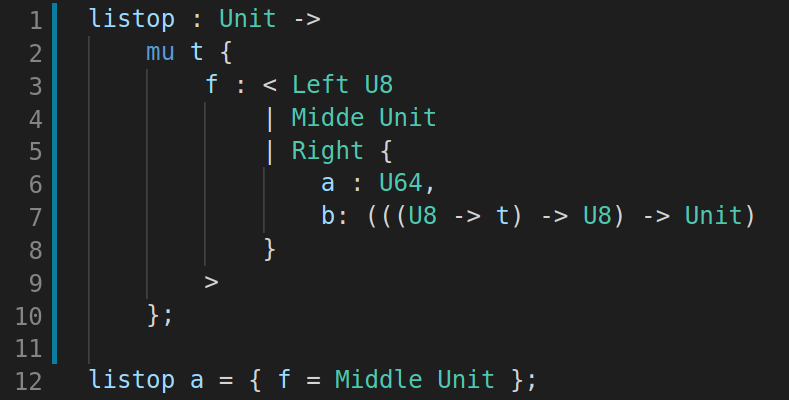
\includegraphics[width=0.8\linewidth]{content/test2.png}
    \caption{A non-strictly positive function}
    \label{fig:test2}
\end{figure}

\begin{figure}
    \centering
    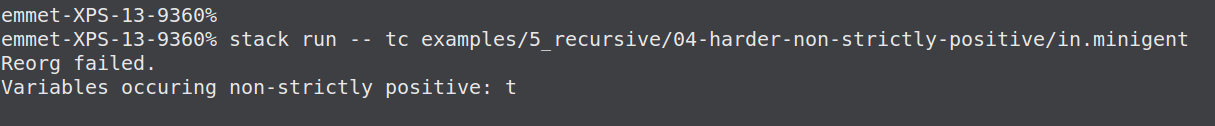
\includegraphics[width=\linewidth]{content/test2result.png}
    \caption{Running the Minigent typechecker on the program in \autoref{fig:test2}}
    \label{fig:test2result}
\end{figure}

\section{Work efficiency}

\todo{talk about syntax highlighting, but also potentially remove?}
